\chapter{积雪的水文过程}
在模式中,覆盖在地表的积雪根据雪盖高度$z_{sno}$被分为最多五层,这种情况下,雪层从上到下分别用$i = −4, −3, −2, −1, 0$编号。编号$i = 0$表示底层,与土壤相邻,$i = snl + 1$表示顶层,其中变量$snl$是雪盖总层数的相反数($-5\leqslant snl\leqslant 0$)。雪层的厚度表示为$\Delta z_i$(m),雪层的深度$z_i$(m)取为其上边界深度$z_{h,i-1}$和下边界深度$z_{h,i}$的中点(由于土壤表面被定义为深度0值,且向下为正,因此雪盖部分的“深度”实际为高度的负值,见图~\ref{fig:模式中积雪雪层示意图})。
{
\begin{figure}[htbp]
\centering
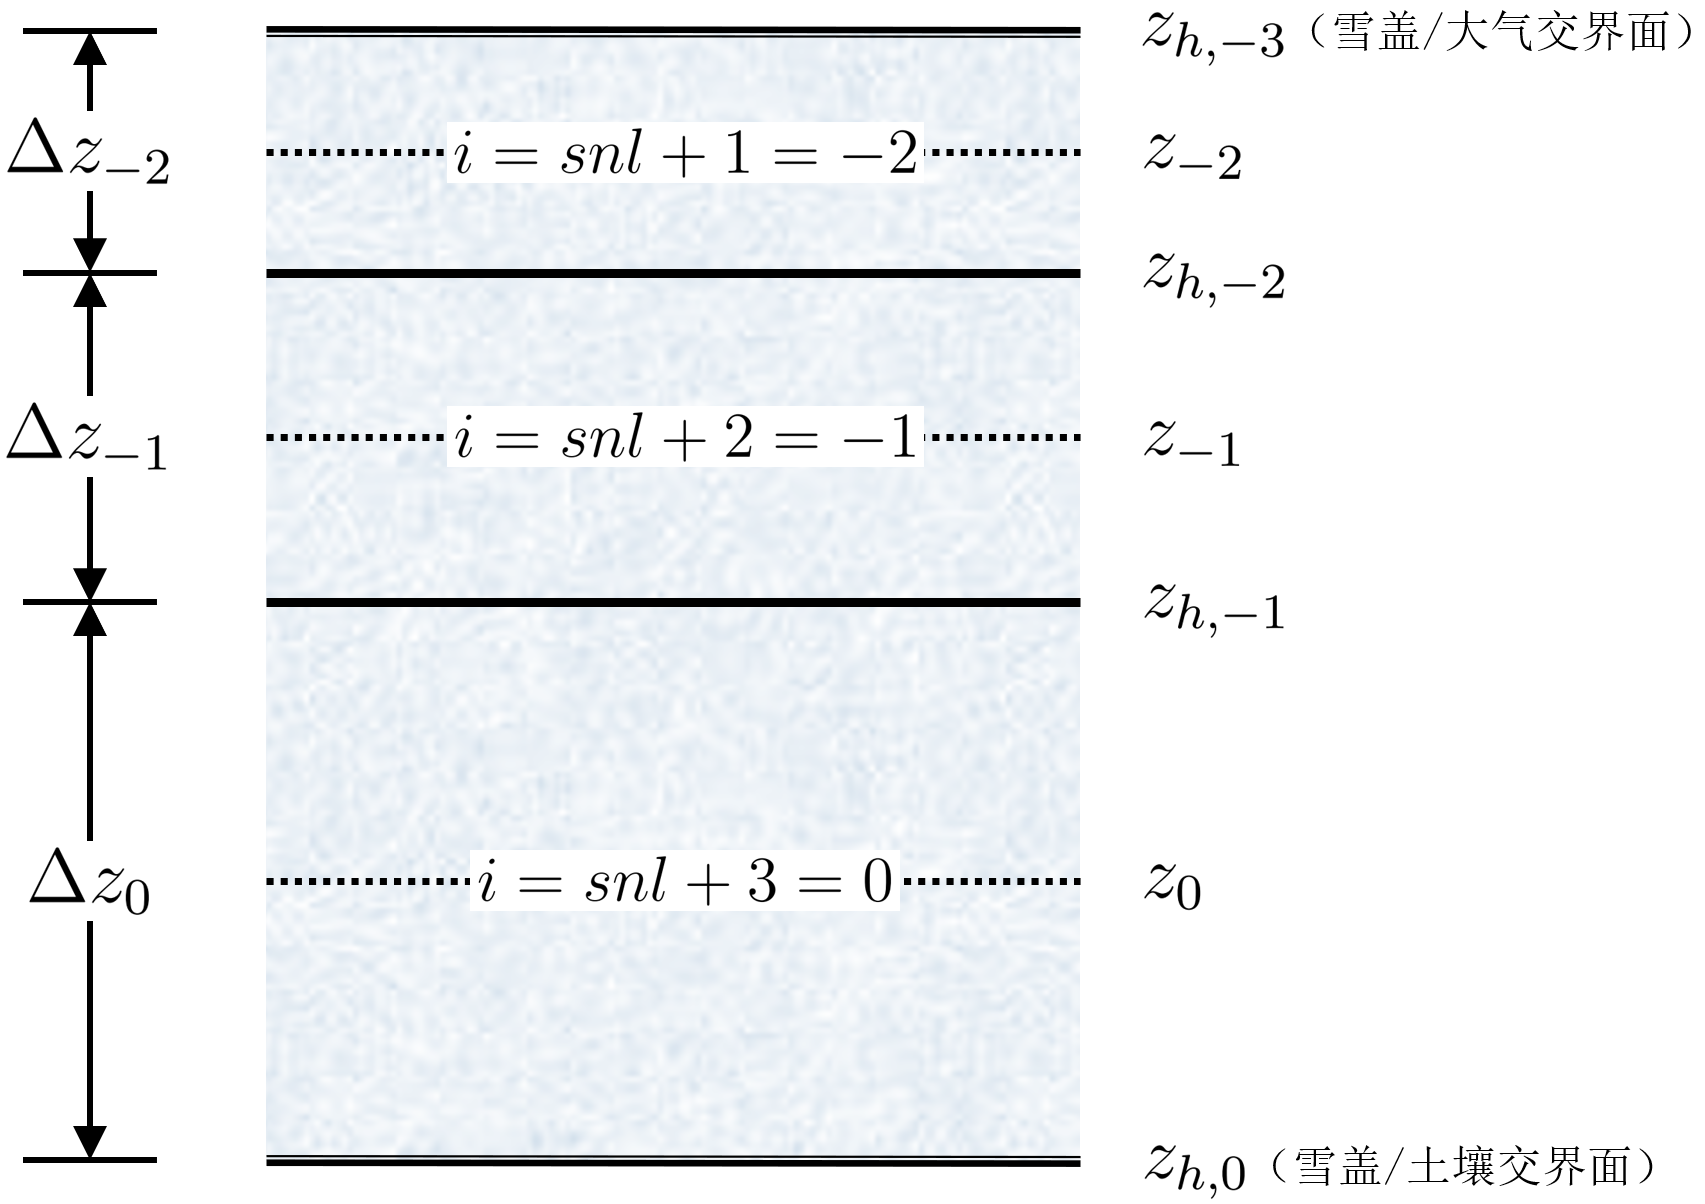
\includegraphics[width=0.8\textwidth]{Figures/雪盖土壤热力过程/模式中积雪雪层示意图.png}
\caption{模式中雪层示意图(以三层为例)}
\label{fig:模式中积雪雪层示意图}
\end{figure}
}
\section{积雪覆盖比例}
\begin{mymdframed}{代码}
    本节对应的代码文件为\texttt{MOD\_SnowFraction.F90}。
\end{mymdframed}

陆地表面可分为被积雪覆盖与未被积雪覆盖两部分。根据 \citet{swenson2012new}提供的方法,
被积雪覆盖的地表面积比例$f_{sno}$可分为两步计算:在积分开始时若有固态降水发生,则新一步的$f_{sno}$更新为
\begin{equation}
f_{{sno }}^{(n+1)}=1-\left[1-\tanh\left(0.1 p_{i} \Delta t\right)\right]\left(1-f_{{sno }}^{(n)}\right) \leqslant 1.0
\end{equation}
其中$p_i$为固态降水速率(\unit{kg.m^{-2}.s^{-1}}),$\Delta t$为积分时间步长(s);在水热过程模拟结束后,若有积雪融化发生,则$f_{sno}$更新为
\begin{equation}
f_{sno}^{(n+1)}=\tanh{\left(\frac{100 z_{s n o}^{2}}{2.5 z_{0 m, s o i} W_{sno}}\right)}
\end{equation}
其中$W_{sno}$为雪水当量(mm),$z_{0m,soi}$ 为未被积雪覆盖时的地表粗糙度。

当植被被积雪掩埋时,已知植被粗糙度$z_{0mv}$,则被积雪掩埋的植被占总植被的比例计算为
\begin{equation}
wt=\frac{0.1 z_{{sno}}}{z_{0mv}+0.1 z_{{sno}}}
\end{equation}
其中$z_{sno}$表示积雪厚度(m)。CoLM2014及以前版本计算斑块中的有效植被比例$f_{sig}=\left(1-wt\right)f_{veg}$,无植被覆盖比例为$\left(1-f_{sig}\right)$。CoLM2024版本为了考虑与PFT次网格类型的兼容性,同时认为积雪是通过覆盖或掩埋植被叶面积、茎面积进行影响,将$wt$用于修正被积雪掩盖后的SAI,即${\rm SAI=TSAI}\left(1-wt\right)$,TSAI为植被“真实”茎面积指数。当采用卫星遥感LAI时,由于其数值已经是非积雪覆盖下的绿色叶面部分,故在此不对其进行积雪覆盖调整。


\section{雪层的建立}\label{sec:雪层的建立}
\begin{mymdframed}{代码}
本节对应的代码文件为\texttt{MOD\_NewSnow.F90}。
\end{mymdframed}


当固态降水$p_{i}$的发生导致雪盖高度$z_{sno}$大于0.01 m且此时尚无雪盖分层,则将在模拟开始时创建一个新的雪层,相关物理量设置如下:
\begin{equation}
\begin{aligned}
& \Delta z_{0} &&= &{z}_{sno}& \\
& z_0 &&= &-0.5\Delta z_0& \\
& z_{h,-1} &&= &-\Delta z_0& \\
& T_0 &&= &\min \left(T_f,T_{atm}\right)& \\
& w_{ice,0} &&= &W_{sno}& \\
& w_{liq,0} &&= &0&
\end{aligned}
\end{equation}
其中$T_f$为液态水凝结温度(~\ref{tab:物理常数}),$T_{atm}$为大气温度,$w_{ice}$和$w_{liq}$分别表示雪层中固态水的含量和液态水的含量(\unit{kg.m^{-2}})。

\section{雪盖中水的垂直运动}\label{雪盖的水量平衡}
\begin{mymdframed}{代码}
本节对应的代码文件为\texttt{MOD\_SoilSnowHydrology.F90}。
\end{mymdframed}

在垂直方向上,雪盖的液态水质量守恒方程为
\begin{equation}
    \frac{\partial w_{liq,i}}{\partial t}=\left(q_{liq,i-1}-q_{liq,i}\right)+\frac{{\left(\Delta w_{liq,i}\right)}_p}{\Delta t}
\end{equation}
其中$q_{liq,i-1}$表示第$i-1$层流入至第$i$层的液态水,$q_{liq,i}$表示第$i$层流出至第$i+1$层的液态水,${{\left(\Delta w_{liq,i}\right)}_p}/{\Delta t}$表示由于相态变化导致的水量改变率(见章节~\ref{sec:温度的相态变化调整})。对于雪盖顶层,需先考虑固态水的变化导致的液态水改变。由于升华和凝华作用,雪盖顶层固态水的变化为
\begin{equation}
    w_{ice,snl+1}^{n+1}=w_{ice,snl+1}^n+\left(q_{frost}-q_{subl}\right)\Delta t
\end{equation}
其中$q_{subl}$和$q_{frost}$分别表示水的升华和凝华速率(\unit{kg.m^{-2}.s^{-1}}或 \unit{mm.H_2O.s^{-1}})。如果$w_{ice,snl+1}^{n+1}<0$,将固态水含量重置为0,并从液态水中减去固态水增加到0所需的水含量。雪盖顶层的$q_{liq,i-1}$则由以下公式计算
\begin{equation}
    q_{liq,i-1}=q_{grnd,liq}+\left(q_{sdew}-q_{seva}\right)
\end{equation}
其中$q_{grnd,liq}$为到达雪盖的液态降水速率,$q_{seva}$和$q_{sdew}$分别表示水的蒸发和凝结速率。基于此,顶层液态水含量更新为
\begin{equation}w_{liq,snl+1}^{n+1}=w_{liq,snl+1}^n+\left(q_{grnd,liq}+q_{sdew}-q_{seva}\right)\Delta t
\end{equation}

当液态水含量超过了雪层的最大持水量时,多余的液态水将下渗到相邻雪层,渗透能力取决于雪层的有效孔隙度($1-\theta_{ice}$)。如果两层中任一层有效孔隙度($1-\theta_{ice,i}$或$1-\theta_{ice,i+1}$)小于不透水体积含水量$\theta_{imp}=0.05$,则假定两层间液态水通量为0。否则,对于雪层$i=snl+1,\ ...,\ 0$,液态水通量$q_{liq,i}$被计算为
\begin{equation}
    q_{liq,i}=\frac{\rho_{liq}\left[\theta_{liq,i}-S_r\left(1-\theta_{ice,i}\right)\right]\Delta z_i}{\Delta t}\geqslant 0
\end{equation}
其中固态水和液态水的体积含水量分别为
\begin{align}
    \theta_{ice,i}&=\frac{w_{ice,i}}{\Delta z_i \rho_{ice}} \leqslant 1 \\
    \theta_{liq,i}&=\frac{w_{liq,i}}{\Delta z_i \rho_{ice}} \leqslant 1-\theta_{ice,i}
\end{align}
$S_r=0.033$称为束缚水饱和度(由于毛细管的滞留作用,渗透结束后雪层仍会保留一定含量的液态水)。$q_{liq,i}$同时也受到相邻下层最大持水量的限制,除非其相邻下层为土壤层,即
\begin{equation}
    q_{liq,i} \leqslant \frac{\rho_{liq}\left(1-\theta_{ice,i+1}-\theta_{liq,i+1}\right)\Delta z_{i+1}}{\Delta t} \qquad i=snl+1,\ ...,\ -1
\end{equation}
于是,液态水含量更新为
\begin{equation}\label{eq:SnowWater}
    w_{liq,i}^{n+1}=w_{liq,i}^n+\left(q_{i-1}-q_i\right)\Delta t
\end{equation}
对于每个时间步长,依次从雪盖顶层到底层计算式~\eqref{eq:SnowWater}。到达土壤层的液态水即为$q_{liq,0}$,被用于地表径流和土壤层的下渗计算当中。

\section{雪盖的黑碳、有机碳和矿物粉尘}
由于大气的气溶胶沉降,积雪中会存在一定的颗粒物,影响雪盖的辐射传输。雪中颗粒物含量仅以质量守恒作为简单约束,这部分的计算均被定义在SNICAR模型中。对于每个雪层,该模型包括了以下八种颗粒物的含量,亲水性黑碳、疏水性黑碳、亲水性有机碳、疏水性有机碳和四种矿物粉尘(颗粒半径分别为0.1-1.0,1.0-2.5,2.5-5.0,5.0-10.0 \unit{\mu m})。每种颗粒物都具有不同的光学属性和融水清除率。

黑碳和有机碳的沉降率被分为以下四类
\begin{align}
    D_{bc,hphob}&=D_{bc,dryphob} \\
    D_{oc,hphil}&=D_{oc,dryhphil}+D_{oc,wethphil} \\
    D_{bc,hphil}&=D_{bc,dryhphil}+D_{bc,wethphil} \\
    D_{oc,hphob}&=D_{oc,dryphob}
\end{align}

假定沉降的颗粒物立即在表面雪层中均匀混合,并在计算雪层层间液态水通量之后添加,以使沉降后的一些气溶胶颗粒位于顶层,并且在进行反照率相关的计算之前不会被冲走。对于每个时间步长,在进行雪层间液态水的垂直运动以及雪层的合并和再分层计算中,都将根据质量守恒更新每层颗粒物含量。每种颗粒物种的质量变化$\Delta m_{sp,i}$为
\begin{equation}
    \Delta m_{sp,i}=\left[k_{sp}\left(q_{liq,i-1} c_{sp,i-1}-q_{liq,i} c_i\right)+D_{sp}\right] \Delta t
\end{equation}
其中$k_{sp}$表示每种颗粒物的融水清除率,具体参见表~\ref{lab:融水清除率}。$c_{sp,i-1}$和$c_{sp,i}$分别表示$i-1$层和$i$层的颗粒物质量混合比(\unit{kg.kg^{-1}}),$D_{sp}$表示大气气溶胶沉降率(仅在$snl+1$层考虑)。颗粒物质量混合比为
\begin{equation}
    c_{i}=\frac{m_{sp,i}}{w_{liq,i}+w_{ice,i}}
\end{equation}

$k_{sp}$的具体值根据~\citet{Conway2012}等人的实验得出。雪盖底层被融水带走的颗粒物被认为从雪盖中永久消失,模式中不再考虑。

\begin{table}[htbp]
    \centering
    \caption{雪盖中不同颗粒物的融水清除率}
    \begin{tabular}{lccc}
    \toprule
        颗粒种类 & $k_{sp}$ \\ \midrule
        亲水性黑碳 & 0.20 \\
        疏水性黑碳 & 0.03 \\
        亲水性有机碳 & 0.20 \\
        疏水性有机碳 & 0.03 \\
        1类矿物粉尘(0.1-1.0 \unit{\mu m}) & 0.02 \\
        2类矿物粉尘(1.0-2.5 \unit{\mu m}) & 0.02 \\
        3类矿物粉尘(2.5-5.0 \unit{\mu m}) & 0.01 \\
        4类矿物粉尘(5.0-10.0 \unit{\mu m}) & 0.01 \\ \bottomrule
    \end{tabular}
    \label{lab:融水清除率}
\end{table}



\section{雪的压实}\label{雪的压实}
\begin{mymdframed}{代码}
本节对应的代码文件为\texttt{MOD\_SnowLayersCombineDivide.F90}。
\end{mymdframed}

积雪的压实主要包括以下四个过程:
\begin{enumerate}
\item 破坏变质作用(新雪的冰晶粒子在风和热力作用下树状结构的破裂),
\item 上覆积雪自重引起的压实,
\item 融化变质作用(积雪经历多次冻融循环后融雪水出流导致雪层结构的改变),
\item 风吹雪引起的压实。
\end{enumerate}

前两个过程的处理方法分别来自 SNTHERM.99 \citep{jordan1999heat}和 SNTHERM.89 \citep{jordan1991one},融化变质的贡献取决于雪层融化过程中前后时刻固态水的变化率,风吹雪压实则考虑了下降风对雪的影响。积雪的总压实率可写为上述四个过程的和:
%
\begin{equation}
C_{R,i}=\frac{1}{\Delta {z_i}} \frac{\partial \Delta {z_i}}{\partial {t}}=C_{R1,i}+C_{R2,i}+C_{R3,i}+C_{R4,i}
\end{equation}
当雪层达到饱和
\begin{equation}
1-\left(\frac{w_{ice,i}}{ \Delta {z_i} \rho_{ice}}+\frac{w_{liq,i}}{ \Delta {z_i} \rho_{liq}}\right) \leqslant 0.001
\end{equation}
或固态水含量$w_{ice,i}\leqslant0.1$时,不再考虑雪的压实。

经过压实后雪层厚度更新为:
\begin{equation}
\Delta z_i^{n+1}=\Delta z_i^n\left(1+C_{R, i} \Delta t\right)
\end{equation}


\subsection{破坏变质引起的压实}
雪在到达地面后,随即快速变化。在热力作用的影响下,单个雪花原有的树状结构发生破裂,向球状结构演变。这些雪花又会和其他雪花融合生长,使雪粒之间结合得更加紧密,最终发生沉降堆积。对于密度小于 \qty{100}{kg.m^{-3}} 的新雪来说,破坏变质引起的沉降非常重要。雪粒的树状结构会使它们之间产生一种类似于“齿轮咬合”的作用,从而具有一定的强度,这种强度在破坏变质的过程中会逐渐减弱。\citet{anderson1976point}对这一阶段的压实过程提出了以下经验函数:
\begin{equation}\label{eq:DestruciveCompact}
C_{R1,i}=\left[\frac{1}{\Delta {z_i}} \frac{\partial \Delta {z_i}}{\partial {t}}\right]_{\text {destructive}}=-2.777 \times 10^{-6} {c}_{3} {c}_{4} {e}^{-0.04\left(T_f-T\right)}
\end{equation}
其中
\begin{equation}
    c_3=\begin{cases}
        1 &\text{当}\ \frac{w_{ice,i}}{\Delta z_i} \leqslant 100 \;\unit{kg.m^{-3}}\text{ 时} \\
        e^{-0.046\left(\frac{w_{ice,i}}{\Delta z_i}-100\right)} &\text{当}\ \frac{w_{ice,i}}{\Delta z_i}>100 \;\unit{kg.m^{-3}}\text{ 时}
    \end{cases}
\end{equation}
\begin{equation}
    c_4=\begin{cases}
        1 &\qquad \quad \qquad \quad \;\text{当}\ \frac{w_{liq,i}}{\Delta z_i} \leqslant 0.01 \;\unit{kg.m^{-3}}\text{ 时} \\
        2 &\qquad \quad \qquad \quad \;\text{当}\ \frac{w_{liq,i}}{\Delta z_i}>0.01 \;\unit{kg.m^{-3}}\text{ 时}
    \end{cases}
\end{equation}
这两个系数表明,当雪层中固态水的体积密度超过 \qty{100}{kg.m^{-3}} 时,破环变质的速率会有所降低;当雪层中存在一定液态水时,破坏变质的速率将成倍增加。

\subsection{雪层负重引起的压实}
随着积雪的累积,上覆积雪的自重会进一步地压实雪层。上覆雪产生的压力(负重)使雪粒粘结生长速度加快,形成更加有效的堆积形状。在经过前一过程的压实后,这一阶段的压实速率会减慢,主要和雪层的负重压力有关。在低压力范围的季节性积雪内,这一阶段的压实率是负重的线性函数\citep{anderson1976point},即
\begin{equation}\label{eq:OverburdenCompact}
C_{R2,i}=\left[\frac{1}{\Delta {z_i}} \frac{\partial \Delta {z_i}}{\partial {t}}\right]_{\text {overburden}}=-\frac{P_{s,i}}{\eta}
%=-\frac{{P}_{{s}}}{9 \times 10^{5}} {e}^{-0.08\left(T_f-{T}\right)-0.023 \rho_{{i}} \theta_{{i}}}
\end{equation}
其中$P_{s,i}$是雪层负重的质量(\unit{kg.m^{-2}}),等于其上覆雪层中固态水和液态水的质量总和加上该层自身固态水和液态水质量的一半,即
\begin{equation}
P_{s,i}=\frac{w_{ice,i}+w_{liq,i}}{2}+\sum_{{j}={snl}+1}^{{j}={i}-1}\left({w}_{ice,j}+{w}_{liq,j}\right)
\end{equation}
~\eqref{eq:OverburdenCompact} 式中变量$\eta$为粘滞系数(\unit{kg.s.m^{-2}}),与雪层的密度和温度有关:
\begin{equation}
    \eta=f_1 f_2 \eta_0 \frac{\rho_i}{c_\eta} e^{a_\eta \left(T_f-T_i\right)+b_\eta \rho_i}
\end{equation}
其中$\rho_i=\frac{w_{ice,i}}{\Delta z_i}$为雪层中固态水的体积密度,常系数$\eta_0=7.62237 \times 10^6$ \unit{kg.s^{-1}.m^{-2}},$a_\eta=0.1$ \unit{K^{-1}},$b_\eta=0.023$ \unit{m^{-3}.kg^{-1}},$c_\eta=450$ \unit{kg.m^{-3}} \citep{Kampenhout2017}。系数$f_1$和雪层中液态水的含量有关~\citep{Vionnet2012}:
\begin{equation}
    f_1=\frac{1}{1+60\frac{w_{liq,i}}{\rho_{liq}\Delta z_i}}
\end{equation}
系数$f_2$则与雪层中棱状雪粒(angular grains)的含量有关,目前的计算中固定$f_2=4$。

\subsection{雪层融化引起的压实}
在融雪过程的后期(积雪经过多次冻融循环后),融雪水的出流导致雪堆更加致密,雪层产生压实。这一阶段的压实率取决于雪层融化过程中前后两个时间步数固态水的变化率
\begin{equation}
C_{R3,i}=\left[\frac{1}{\Delta {z_i}} \frac{\partial \Delta {z_i}}{\partial {t}}\right]_{\text{melt}}=-\frac{1}{\Delta {t}}\max\left(0,\frac{{f}_{{ice,i}}^{n}-{f}_{{ice,i}}^{n+1}}{{f}_{ice,i}^{n}}\right)
\end{equation}
其中$f_{ice,i}=w_{ice,i}/\left({w_{ice,i}+w_{liq,i}}\right)$为雪层中固态水占全部水含量的比例。

\subsection{风吹雪引起的压实}
在高纬的冰原地区,低温使破坏变质的过程发生缓慢,此时高速的下降风将占据主导,气流使雪粒的树状结构破碎,引发雪粒堆积,产生压实。在这种情况下,引入风吹雪压实的参数化方案~\citep{Vionnet2012}:
\begin{equation}
    C_{R4,i}=\left[\frac{1}{\Delta z_i}\frac{\partial \Delta z_i}{\partial t}\right]_{\text{drift}}=-\frac{\max \left(0,\rho_{\text{max}}-\rho_i\right)}{\tau_i}
\end{equation}
其中,$\rho_{\text{max}}=350$ \unit{kg.m^{-3}}是这一过程的有效密度上限,$\tau_i$是一个与雪层深度有关的时间尺度变量:
\begin{equation}
    \tau_i=\frac{\tau}{\Gamma_{\text{drift}}^i}, \quad \Gamma_{\text{drift}}^i=\max \left(0,S_I^i e^{-z_i/0.1}\right)
\end{equation}
常数$\tau$是风吹雪压实过程的一个特征时间尺度,根据经验被设置为48 \unit{h},$z_i=\sum_j \Delta z_j \cdot \left(3.25-S_I^j\right)$称为伪深度,与当前雪层$i$上方的$j$个雪层的硬化程度有关。$S_I$称为吹雪飘移指数(driftability index):
\begin{equation}
    S_I=-2.868 e^{-0.085 U} + 1 + M_O
\end{equation}
其由10 \unit{m}风速$U$和雪的流动指数(mobility index)$M_O$共同作用,反映了雪粒在风的作用下受到的飘移影响。雪的流动指数
\begin{equation}
    M_O=0.34\left(-0.583g_s-0.833s+0.833\right)+0.66F\left(\rho\right)
\end{equation}
与雪的微观结构有关,描述了雪层受侵蚀的可能性,其中
$$F\left(\rho\right)=1.25-0.0042 \cdot \\\left[\max \left(\rho_{min},\rho\right)-\rho_{min}\right],$$$\rho_{min}=50$ \unit{kg.m^{-3}}。$g_s$和$s$是两个和雪粒形态有关的变量,$s$称为雪粒的球度(sphericity),从0 -- 1不等,$g_s$为雪粒大小,一般为0.3至0.4 \unit{mm}。


\section{雪层的合并}\label{雪层的合并}
\begin{mymdframed}{代码}
本节对应的代码文件为\texttt{MOD\_SnowLayersCombineDivide.F90}。
\end{mymdframed}

雪层的合并包括以下两种情况:1.考虑固态水的含量。当任何一层几近融化(即$w_{ice,i} \leqslant 0.1$ \unit{kg.m^{-2}})时,移除该雪层,且将其液态水和固态水含量分配到与之相邻的下层中:
\begin{equation}
    w_{liq,i+1} = w_{liq,i+1} + w_{liq,i}
\end{equation}
\begin{equation}
    w_{ice,i+1} = w_{ice,i+1} + w_{ice,i}
\end{equation}
这也包括了与土壤相邻的底层雪层,该层的液态水和固态水含量将直接被分配到土壤层顶层中。每移除一层雪层,该层以上的雪层编号将增加1,该层以下的雪层编号保持不变,以对应新的雪盖分层。

此时,如果已无雪层存在($snl=0$),雪水当量$W_{sno}$和雪盖高度$z_{sno}$将被设为0。如果仍有雪层存在,则$W_{sno}$和$z_{sno}$根据下式更新为
\begin{equation}
    W_{sno} = \sum_{i=snl+1}^{i=0}\left(w_{ice,i}+w_{liq,i}\right)
\end{equation}
\begin{equation}
    z_{sno} = \sum_{i=snl+1}^{i=0} \Delta z_i
\end{equation}
若雪盖高度$z_{sno} < 0.01$ \unit{m},则雪盖层数$snl$仍被设为0,此时雪水当量
$$W_{sno}=\sum_{i=snl+1}^{i=0} w_{ice,i}$$
将仅计算雪盖固态水含量,雪盖液态水含量$\sum_{i=snl+1}^{i=0} w_{liq,i}$将分配给土壤层顶层。

2.考虑雪层的厚度。当某一雪层的厚度$\Delta z_i$小于规定的最小值$\Delta z_{min}$时,则将该雪层与相邻雪层合并。如果该雪层:
\begin{enumerate}
\item 为顶层,则与相邻的下层雪层合并;
\item 为底层(与土壤相邻),则与相邻的上层雪层合并;
\item 为中间层,则与厚度较薄的相邻雪层合并。
\end{enumerate}

五个雪层(从顶层到底层)规定的厚度最小值$\Delta z_{min}$分别为 0.010、0.015、0.025、0.055 和 0.115 \unit{m}。

当两个雪层(这里用编号1和2表示)合并时,合并层的厚度为
\begin{equation}\label{eq:SnowCombThick}
\Delta {z}_c=\Delta {z}_{1}+\Delta {z}_{2}
\end{equation}
根据质量守恒,合并层的质量计算为
\begin{equation}
w_{liq,c}=w_{liq,1}+w_{liq,2}
\end{equation}
\begin{equation}
w_{ice,c}=w_{ice,1}+w_{ice,2}
\end{equation}
根据焓变守恒,合并层的温度计算为
\begin{equation}\label{eq:SnowCombTemp}
T_c=\begin{cases}
    T_f+{h_c}/\left(C_{ice}w_{ice,c}+C_{liq}w_{liq,c}\right) &\text{当}\ h_c<0 \text{ 时} \\
    T_f &\text{当}\ 0 \leqslant h_c \leqslant L_f w_{liq,c} \text{ 时}\\
    T_f+\left(h_c-L_f w_{liq,c}\right)/\left(C_{ice} w_{ice,c}+C_{liq} w_{liq,c}\right) &\text{当}\ h_c > L_f w_{liq,c} \text{ 时}
\end{cases}
\end{equation}
其中$h_c=h_1+h_2$为两个雪层合并后的焓,第$i$层的焓$h_i$可通过以下公式得出
\begin{equation}
    h_i=\left(C_{ice}w_{ice,i}+C_{liq}w_{liq,i}\right)\left(T_i-T_f\right)+L_fw_{liq,i}
\end{equation}
$L_f$为固态水融化潜热,$C_{liq}$和$C_{ice}$分别为液态水和固态水的比热容(表~\ref{tab:物理常数})。

最后,根据下式更新雪层深度和雪层交界面深度
\begin{equation}
    z_i=z_{h,i}-0.5\Delta z_i \;\;\;\;\;i=0,\;...,\;snl+1
\end{equation}
\begin{equation}
    z_{h,i-1}=z_{h,i}-\Delta z_i \;\;\;\;\;i=0,\;...,\;snl+1
\end{equation}



\section{雪层的再分层}\label{雪层的再分层}
当某一雪层的厚度$\Delta z_i$大于规定的最大值$\Delta z_{max}$时,该雪层将被再分。最大厚度$\Delta z_{max}$和雪盖的层数有关。例如,如果雪盖只被分为一层,那么顶层(也就是该层)的最大厚度将为0.03 \unit{m};如果雪盖被分为多层,那么顶层的最大厚度则为0.02 \unit{m}。不同情况雪层的最大厚度如图~\ref{fig:不同情况下雪层的最大厚度}所示。

{
\begin{figure}[htbp]
\centering
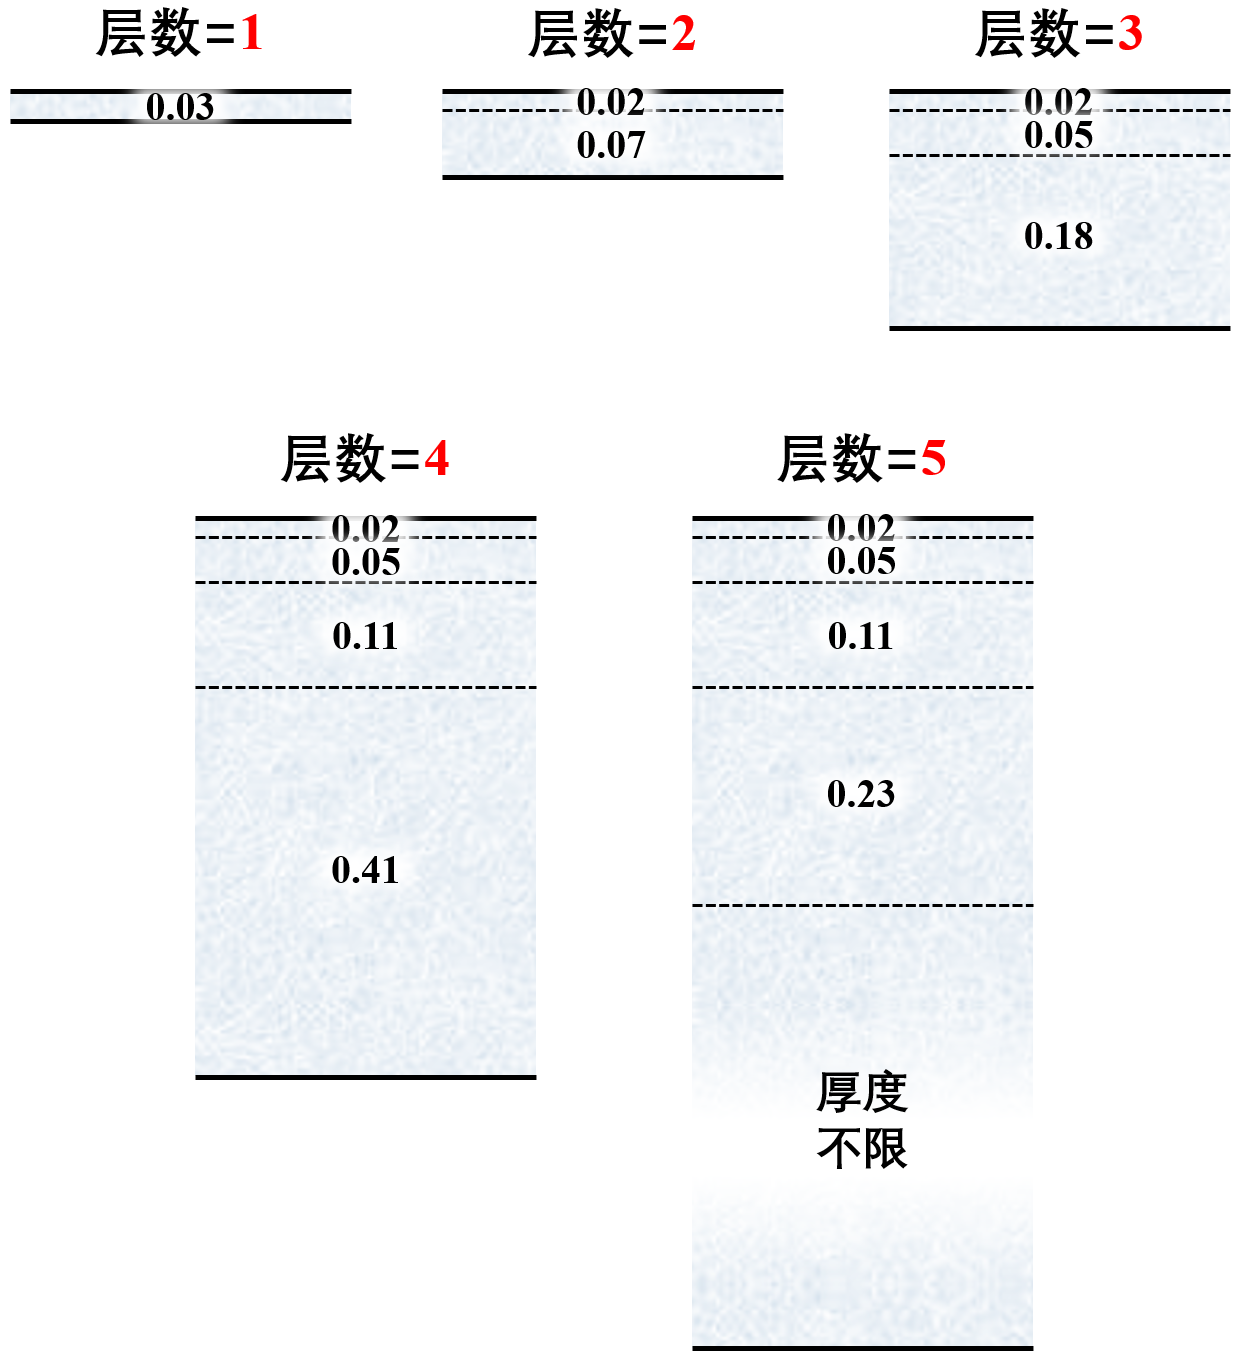
\includegraphics[width=0.6\columnwidth]{Figures/雪盖土壤热力过程/不同情况下雪层的最大厚度.png}
\caption{不同情况下雪层的最大厚度示意图}
\label{fig:不同情况下雪层的最大厚度}
\end{figure}
}

如果被再分的雪层为底层,则将该雪层等分为厚度相等的两层,并均分液态水含量和固态水含量,温度和原雪层保持一致,此时雪盖总层数将增加1(即$snl$将减少1)。如果被再分的雪层不为底层,先将该层分为上下两层,其中上层雪层的厚度限为该层的规定最大厚度$\Delta z_{max}$,下层雪层的厚度则为$\Delta z_i - \Delta z_{max}$,原雪层的液态水含量和固态水含量按厚度比例分配给上下两个雪层,温度在再分前后保持不变,再将下层雪层作为多余部分根据式~\eqref{eq:SnowCombThick} -~\eqref{eq:SnowCombTemp}和原雪层的相邻下层雪层合并,从而保证雪盖总层数不变。

如图~\ref{fig:以三层为例雪层再分层的方法},假设某一时间步,模式中包含三层雪层,其厚度从上至下分别为0.02、0.08和0.17 m,参考图~\ref{fig:不同情况下雪层的最大厚度}中三层情况下的最大厚度标准考虑,则第$i=-1$层厚度$\Delta z_{-1}=0.08 > \Delta z_{max,-1}=0.05 $,此时将其厚度截取0.03 m分配至相邻下层雪盖,使其厚度减少为$\Delta z_{-1}=0.05$,刚好满足最大阈值。这时,底层雪盖厚度将增加为$\Delta z_{0}=0.20$,同样超过了$\Delta z_{max,0}=0.18$,则将该层再次划分为厚度相等的两层,均为0.10 m。于是,总雪盖层数便增加至四层,每层厚度如图中所标注,之后的计算则以四层为标准。

{
\begin{figure}[htbp]
\centering
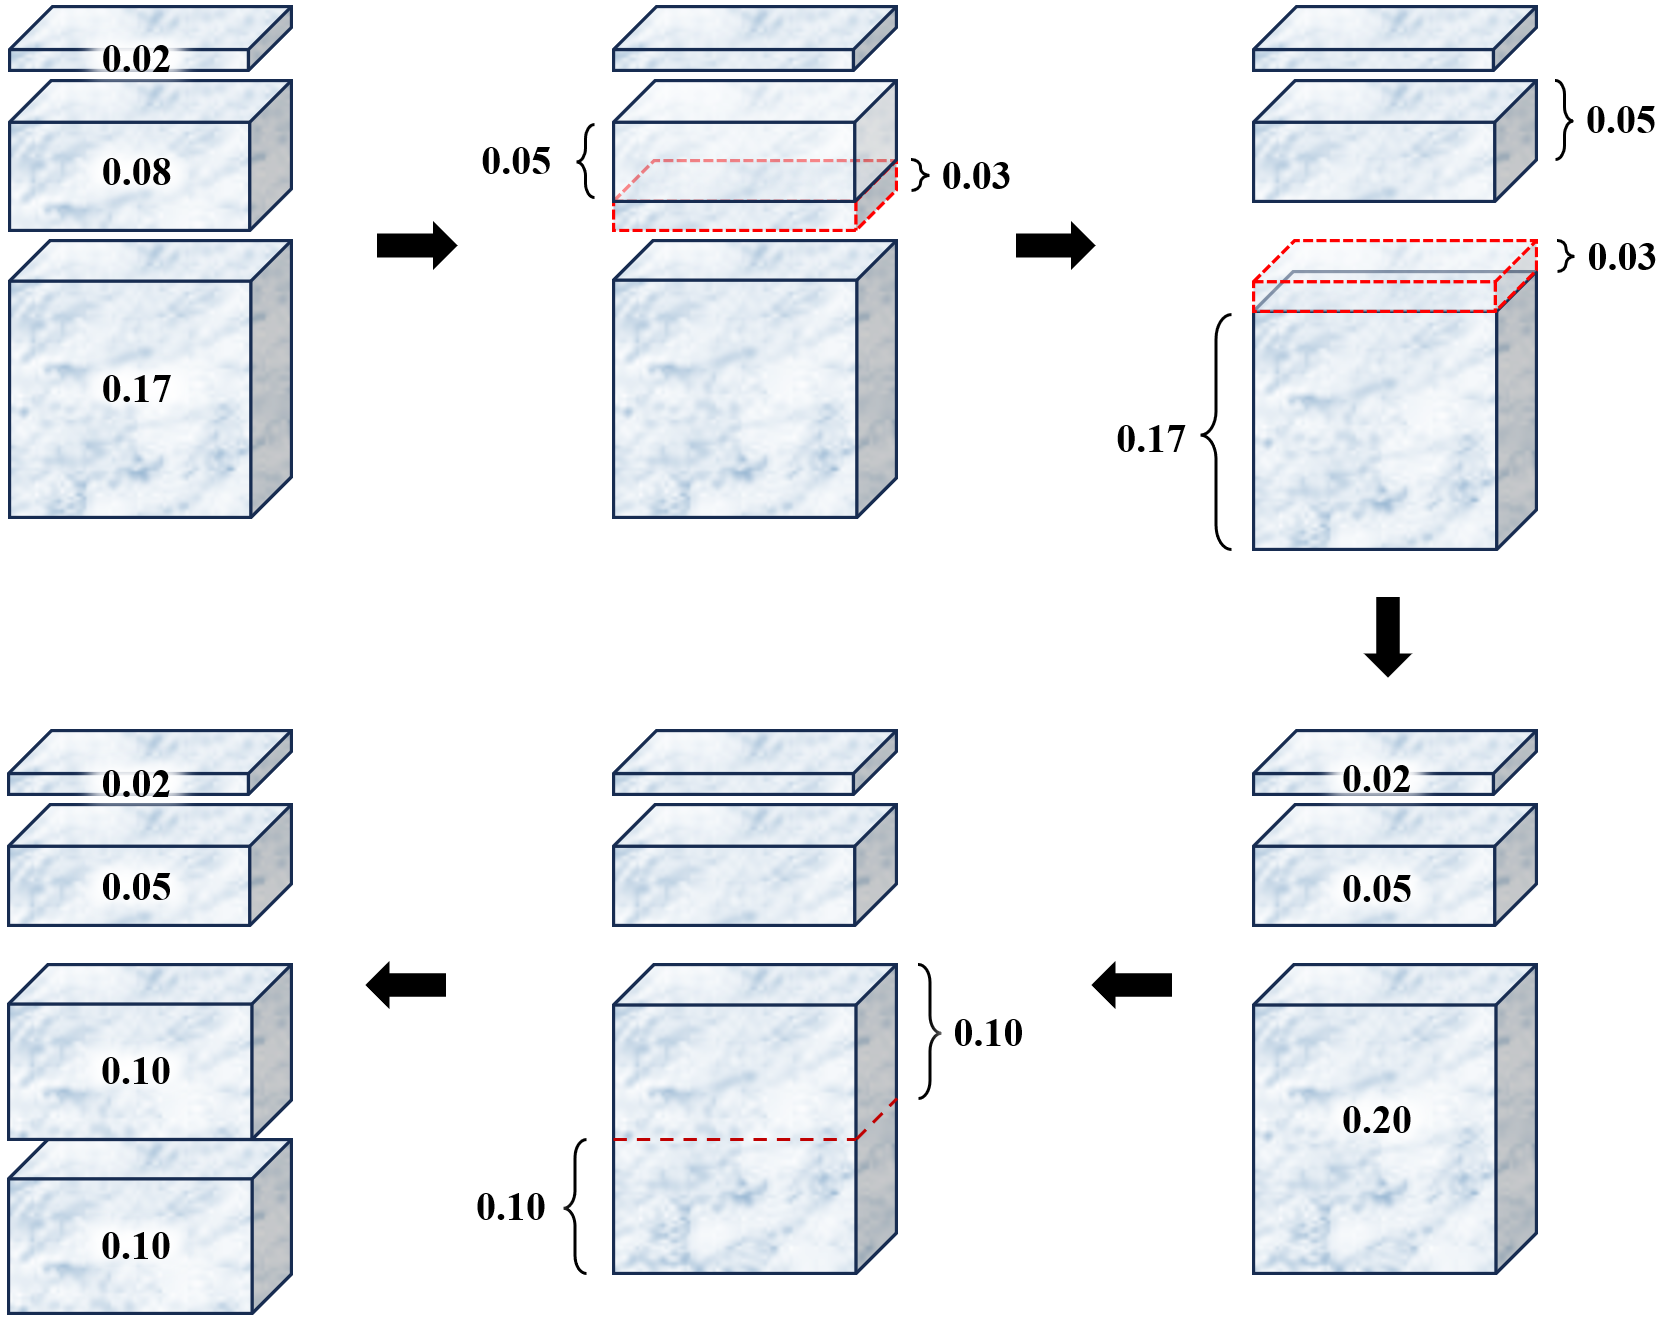
\includegraphics[width=0.6\columnwidth]{Figures/雪盖土壤热力过程/以三层为例雪层再分层的方法.png}
\caption{以三层为例,雪层再分层的方法示意图}
\label{fig:以三层为例雪层再分层的方法}
\end{figure}
}


